% This version of CVPR template is provided by Ming-Ming Cheng.
% Please leave an issue if you found a bug:
% https://github.com/MCG-NKU/CVPR_Template.

% \documentclass[review]{cvpr}
\documentclass[final]{cvpr}

\usepackage{times}
\usepackage{epsfig}
\usepackage{graphicx}
\usepackage{amsmath}
\usepackage{amssymb}

% Include other packages here, before hyperref.

% If you comment hyperref and then uncomment it, you should delete
% egpaper.aux before re-running latex.  (Or just hit 'q' on the first latex
% run, let it finish, and you should be clear).
\usepackage[pagebackref=true,breaklinks=true,colorlinks,bookmarks=false]{hyperref}


\def\confYear{CVPR 2021}
%\setcounter{page}{4321} % For final version only


\begin{document}

%%%%%%%%% TITLE
\title{The Report of the Assignment 2:\\Implementing and Reproducing MAML and REPTILE}

\author{Seungmin Lee\\
Seoul National University\\
{\tt\small dltmdals14@snu.ac.kr}
}

\onecolumn
\maketitle


%%%%%%%%% BODY TEXT
\section{Introduction}
In this assignment, I implemented and reproduced MAML~\cite{maml}, FOMAML~\cite{maml} and Reptile~\cite{reptile}. I followed the instructions for all experiments. Therefore, I will skip all the details of experiments. The reported hyperparameters in papers are not helpful, so I should re-search all the hyperparameters, which requires too many time. 

\section{Omniglot Classification Results}~\label{omniglot}
In Omniglot~\cite{omniglot} experiments, we compare just FOMAML~\cite{maml} and Reptile~\cite{reptile}. The results can be shown in Figure~\ref{comp2}. As we can see in the figure, 1-shot and 5-shot results are similar in that they are converge very fastly. However, the starting losses are quite different. More specifically, in 1-shot classification, the starting loss of FOMAML is between 4 and 5, while that of 5-shot classification is larger than 7. In other hand, the results of Reptile show similar in both experiments. The final losses of FOMAML is smaller than that of Reptile. Moreover, the accuracies of FOMAML is larger than Reptile. The final accuracies of FOMAML are 92.29 and 96.58 for 1-shot and 5-shot classification, respectively, while the final accuracies of Reptile are only 87.21 and 87.30.

\begin{figure}[b]
    \centering
	\begin{tabular}{c}
		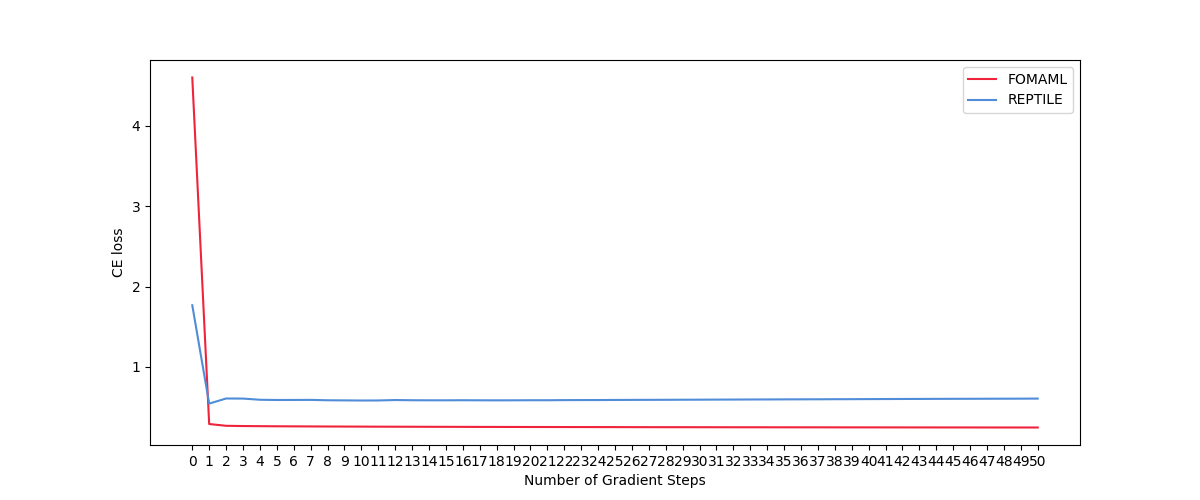
\includegraphics[width=0.9\textwidth]{resources/omniglot_5way_1shot.png}\\
		(a) 5-way 1-shot classification\\
		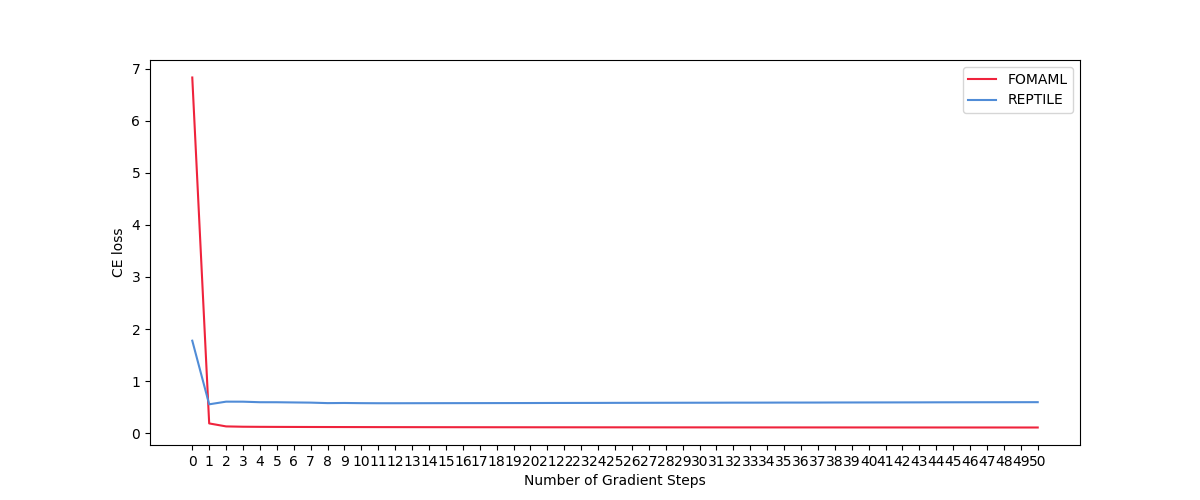
\includegraphics[width=0.9\textwidth]{resources/omniglot_5way_5shot.png}\\
		(b) 5-way 5-shot classification\\
	\end{tabular}\vspace{0.2cm}
	\caption{The results of (a) 5-way 1-shot classification and (b) 5-way 5-shot Omniglot classification.}
	% \vspace{-0.4cm}
	\label{comp2}
\end{figure}


\section{Sine Waves Regression Results}
As we can see in the previous section~\ref{omniglot}, the implementations of the alogrithms are fine. However, tuning hyperparameters on this regression tasks requires too many resources. The results are shown in Figure~\ref{sin5} and Figure~\ref{sin10}. For 5-shot tasks, the training losses first increase then decrease. These results show that the learning is not doen well. For 10-shot tasks, the losses decrease monotonically. However, the difference between updating 1 step and 5 steps is small.

\begin{figure}[b]
    \centering
	\begin{tabular}{c}
		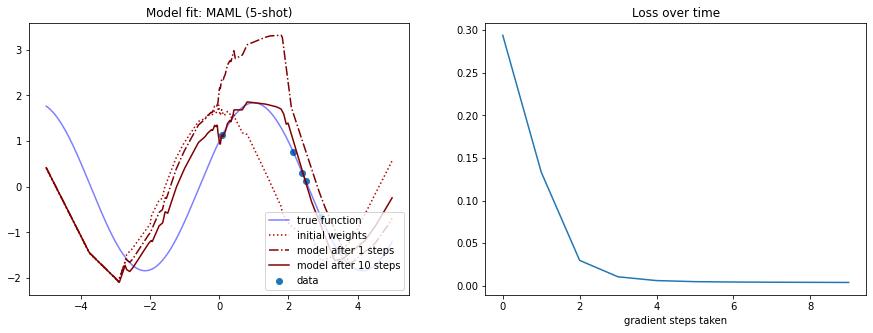
\includegraphics[width=0.9\textwidth]{resources/maml_5.png}\\
		(a) MAML (5-shot) \\
		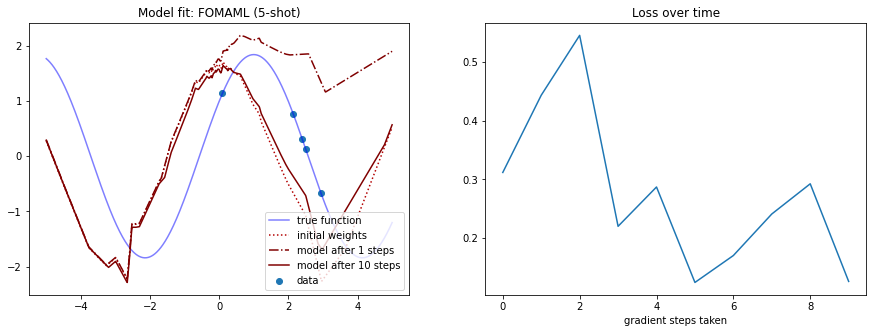
\includegraphics[width=0.9\textwidth]{resources/fomaml_5.png}\\
		(a) FOMAML (5-shot) \\
		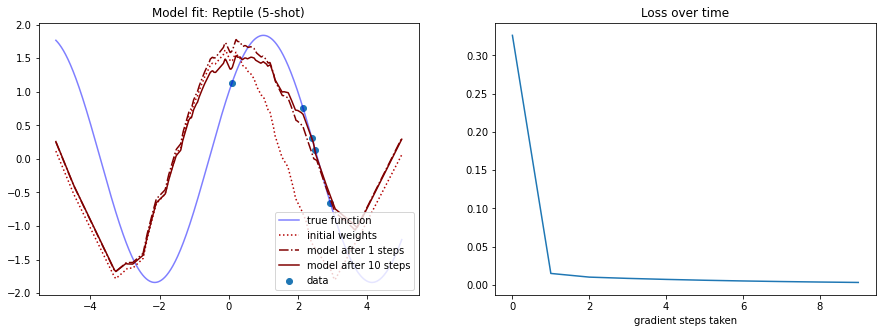
\includegraphics[width=0.9\textwidth]{resources/reptile_5.png}\\
		(a) Reptile (5-shot) \\
	\end{tabular}\vspace{0.2cm}
	\caption{The results of 5-shot sine waves regression tasks.}
	% \vspace{-0.4cm}
	\label{sin5}
\end{figure}

\begin{figure}[b]
    \centering
	\begin{tabular}{c}
		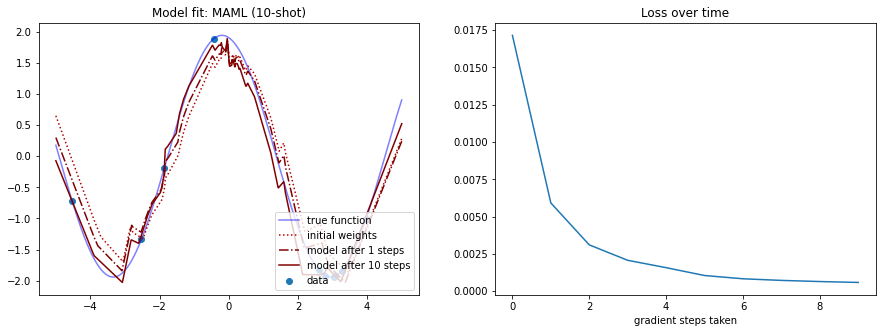
\includegraphics[width=0.9\textwidth]{resources/maml_10.png}\\
		(a) MAML (10-shot) \\
		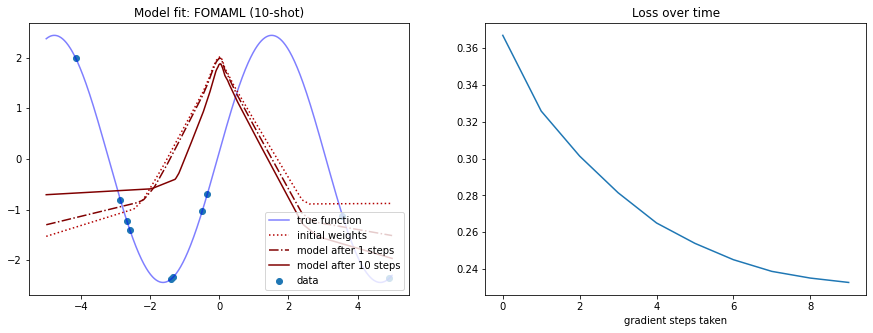
\includegraphics[width=0.9\textwidth]{resources/fomaml_10.png}\\
		(a) FOMAML (10-shot) \\
		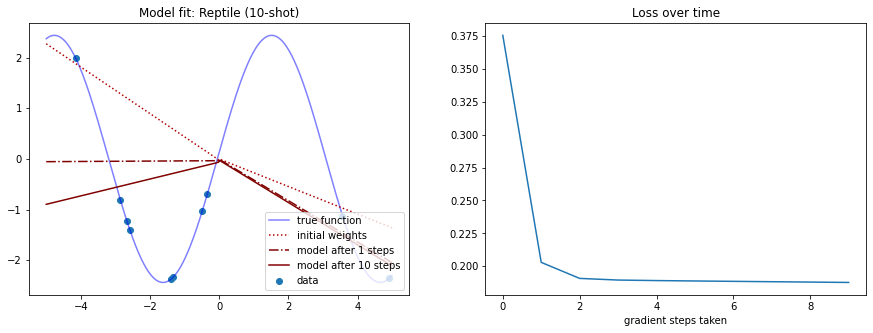
\includegraphics[width=0.9\textwidth]{resources/reptile_10.png}\\
		(a) Reptile (10-shot) \\
	\end{tabular}\vspace{0.2cm}
	\caption{The results of 10-shot sine waves regression tasks.}
	% \vspace{-0.4cm}
	\label{sin10}
\end{figure}

{\small
\bibliographystyle{ieee_fullname}
\bibliography{egbib}
}

\end{document}
